% Text:              X
% Citations:         X
% Revision:          X
% Final Revision:    X
\chapter{Using the Visualization Tool}
With the foundational knowledge and context for the microservice architecture, microservice patterns, the Jolie programming language, and the current tools both for Jolie and for visualization in general in place, it is time to get familiar with the tool developed for this thesis.

This chapter will go into how the tool is used to enhance the development experience by going through a simple example microservice application.
Firstly, an application is defined. The application for this example is a simple e-commerce platform consisting of seven microservices:

\begin{itemize}
    \item \textbf{User service} - Handles user authentication. Lets the client create, update and delete their account and also log in to get an authentication token.
    \item \textbf{Product service} - Handles product information. This service exposes a basic CRUD (Create Read Update Delete) API for products sold on the platform.
    \item \textbf{Recommended service} - Handles fetching recommended products. A client can query this service which will, based on the user's id, return a list of products which the user might also like.
    \item \textbf{Order service} - Handles grouping of selected products and all the information required for the user to place an order. This includes shipping and tax fees.
    \item \textbf{Payment service} - Handles transactions of orders. When the user places an order they must provide some kind of payment method as well as the necessary information to complete the transaction.
    \item \textbf{Analytics service} - A monitoring service. This service can keep track of popular products, frequent shoppers, what products get bought together, and much more.
    \item \textbf{Notification service} - Handles sending e-mails to users when the transaction is approved. Can also send promo codes, offers, and discounts to users.
\end{itemize}
This example is very simplified, and only the architectural aspect of the microservices will be implemented, meaning the connections between services and the APIs. This means that no business logic will be implemented, and
the types of interface operations will be heavily simplified since the functionality of the application is not what is in focus in this chapter.
Other details such as deployment, data persistence, and security will also be omitted from this example. A simple diagram can be seen in figure \ref*{figure:full_example_lc} which displays the desired architecture of the application.

To showcase the visualization capabilities of the tool the application will not be developed using any architectural programming features from Jolie such as embeddings, aggregation, redirection, etc.
These will, however, be introduced at a later point.

\begin{figure}[h!]
    \center
    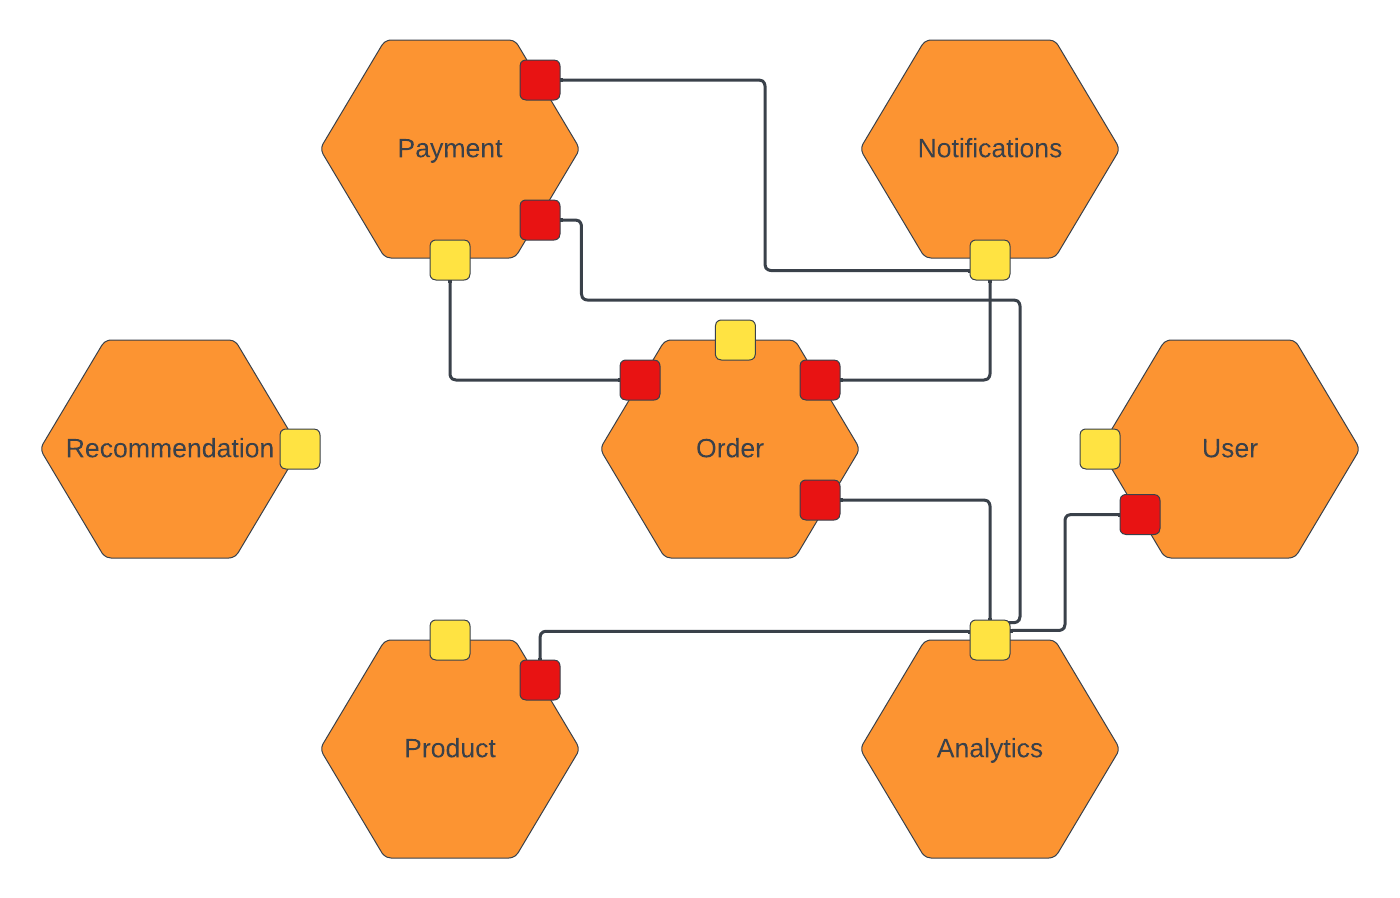
\includegraphics[width=0.70\textwidth]{figures/full_example_lc.png}
    \caption{A diagram of the example architecture of the e-commerce application. The output ports (red) represent internal communication between the services via their input ports (yellow).}
    \label{figure:full_example_lc}
\end{figure}

\section{Setup and Requirements}
In order to use the tool, Jolie must be set up correctly with version \texttt{1.11.0-git}. This section will not specify how this is done, but the Jolie website goes more in detail on how
the correct git version is installed. From this point onwards it is assumed that the environment variables are set correctly to point to the git version of Jolie.

The tool is developed to be used with Visual Studio Code, aka VS Code, which is a code editor developed by Microsoft.
VS Code has a large ecosystem of plugins which are used to enhance the developing experience.
To start using the tool, it must be downloaded and installed either from the VS Code marketplace under the name: \texttt{\toolname}, or compile the source code and extract a \texttt{.VSIX} file to install manually.

The development starts with creating a \texttt{.JSON} file which \toolname[] uses to know which services are at the top level of the application.
The plugin has a default file name it will look for, namely, \texttt{architecture.jolie.json} located in the root folder, which is where the developer will define all top-level services, networks, and properties of the services.
The plugin comes with a command to initialize the architecture file, and this creates the file and populates it with a template service contained in a network.

\subsection{Structure of the Architecture File}
The architecture file is a JSON file which consists of an array of arrays of services. The outermost array can semantically be understood as the list of all networks.
Listing \ref*{lst:architecture-file-structure} shows this structure where the \texttt{\{...\}} represents the services. Each network can have any number of services, and it is up to the
developer to specify what a network represents depending on where the services will deploy.

\begin{jsonlisting}[][caption={Structure of the architecture JSON file showing two networks.}, label=lst:architecture-file-structure]
[
    [
        { "file": "svc1.ol" }
    ],
    [
        { "file": "svc2.ol" }
    ]
]
\end{jsonlisting}

The services have different properties which the user can specify. All properties are showcased in appendix \ref*{appen:architecture-file-structure}.
For the example in this chapter, only the file needs to be specified for each service.

\section{Developing the Services}
All seven services in this example will have a unique folder each in the root directory of the project. This is done to separate which files are belongs the which service.
In each folder, JPM can be initialized if the developer needs it, and the interfaces, types, and services will all be separated in files as well.

The tool will be utilized as much as possible to create and refactor code, all while every service being developed will be visualized next to the source code in VS Code.
Every time a service has been declared it is added to the architecture file. This can be done quickly by the developer using code snippets added by the tool. All similar quality-of-life improvements will be discussed in another section.
\subsection{The User Service}
The interface which specifies what operations the user service implements is called \texttt{UserIFace} in this example.
Listing \ref*{lst:useriface} shows how the interface is set up. The ErrorResponse type is a more universal response type which gives a message and status code, which can be used in case of an error, but with no error, it will simply set the error flag to false.
Each of the request types represents what data the operation needs to run. For registering users and logging in an email and password are needed. The update request type represents the user to be updated and what is going to be updated for the user. The delete request simply needs the user ID of the user.

\begin{jolisting}[][caption={The interface for the user service}, label={lst:useriface}]
interface UserIFace {
    RequestResponse:
        register(RegisterRequest)(ErrorResponse),
        login(LoginRequest)(LoginResponse),
        updateUser(UpdateRequest)(ErrorResponse),
        deleteUser(DeleteRequest)(ErrorResponse),
}
\end{jolisting}

The service is created in the main file and the execution is set to \textit{concurrent}.
The service can now be added to the architecture file. Since only one service is present in the main OL file, only the file name needs to be specified in the service JSON.
Now the visualization tool can be run using the command \textit{Jolie: Visualize} in VS Code, and a single service called \textit{User} can be seen.

To use the tool to add the ports, double-click on the service to open the service in the sidebar. Next to the empty lists of ports, a \texttt{"+"} button can be clicked to add either an input port or an output port.
This will bring up a pop-up window, shown in figure \ref*{figure:popup_create_inputport}, where the user can specify the details of the port such as name, location, protocol and a list of interfaces.
\begin{figure}[h!]
    \center
    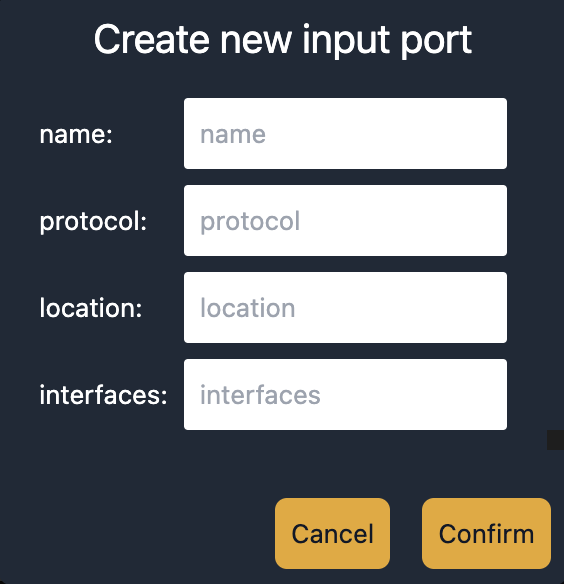
\includegraphics[width=0.35\textwidth]{figures/popup_create_inputport.png}
    \caption{Pop up in the visualization tool where a user can specify details about a port, and by clicking 'confirm' will add that port in code.}
    \label{figure:popup_create_inputport}
\end{figure}

Using this feature. The service needs to have an input port which uses the interface specified before, \texttt{UserIFace}, and before creating the output port for the analytics service, the interface for the analytics service should be defined to prevent a parsing error from the Jolie parser. 
The analytics interface is called \texttt{AnalyticsIFace}, and the operations will be discussed in another section. For now, it is just an empty interface.

After clicking 'confirm' on the popups, the interfaces are correctly imported if they exist. The code for the user service is displayed in
listing \ref*{lst:user-svc}, where some of the implementation details are omitted, but the general structure of the service can be seen.

\begin{jolisting}[][caption={The user service after the ports have been created with omitted implementation details.}, label={lst:user-svc}]
from .userInterface import UserIFace
from ..analytics.analyticsInterface import AnalyticsIFace
service User {

    execution{ concurrent }

    inputPort IP {
        ...
        Interfaces: UserIFace
    }

    outputPort Analytics {
        ...
        Interfaces: AnalyticsIFace
    }

    main {
        ...
    }
}
\end{jolisting}

The implementation details of the types are omitted here but can be seen in Appendix % TODO

\subsection{The Product Service}
The product service handles all operations of the products. This is a basic CRUD service, which also will send analytics to the analytics service, which can be used to monitor popular products etc.
The create and update operation's request types require a product, which is a type containing information about the product, and a user ID because only users who own the product should be able to alter it.
The read operation request type is only an integer corresponding to the product ID. The delete operation request type is a type containing the user ID and product ID to, once again, check if the user is allowed to delete the product and the ID of the product.

When the types and interface (ProductIFace) have been created,
a service named \textit{Product} is created in the main \texttt{.ol} file and once again the execution context is set to \textit{concurrent}.
The tool is added to the architecture file in the same network as the user service, and can now be seen in the visualization user interface.

By opening the product service in the sidebar the input and output port can be created similarly to the user service previously. The input port will use the \texttt{ProductIFace} interface and the output port will use the \texttt{AnalyticsIFace} interface.
The two services displayed in the visualization UI can be seen in figure \ref*{figure:jv_product_and_user} with the two ports created for each service.
\begin{figure}[h!]
    \center
    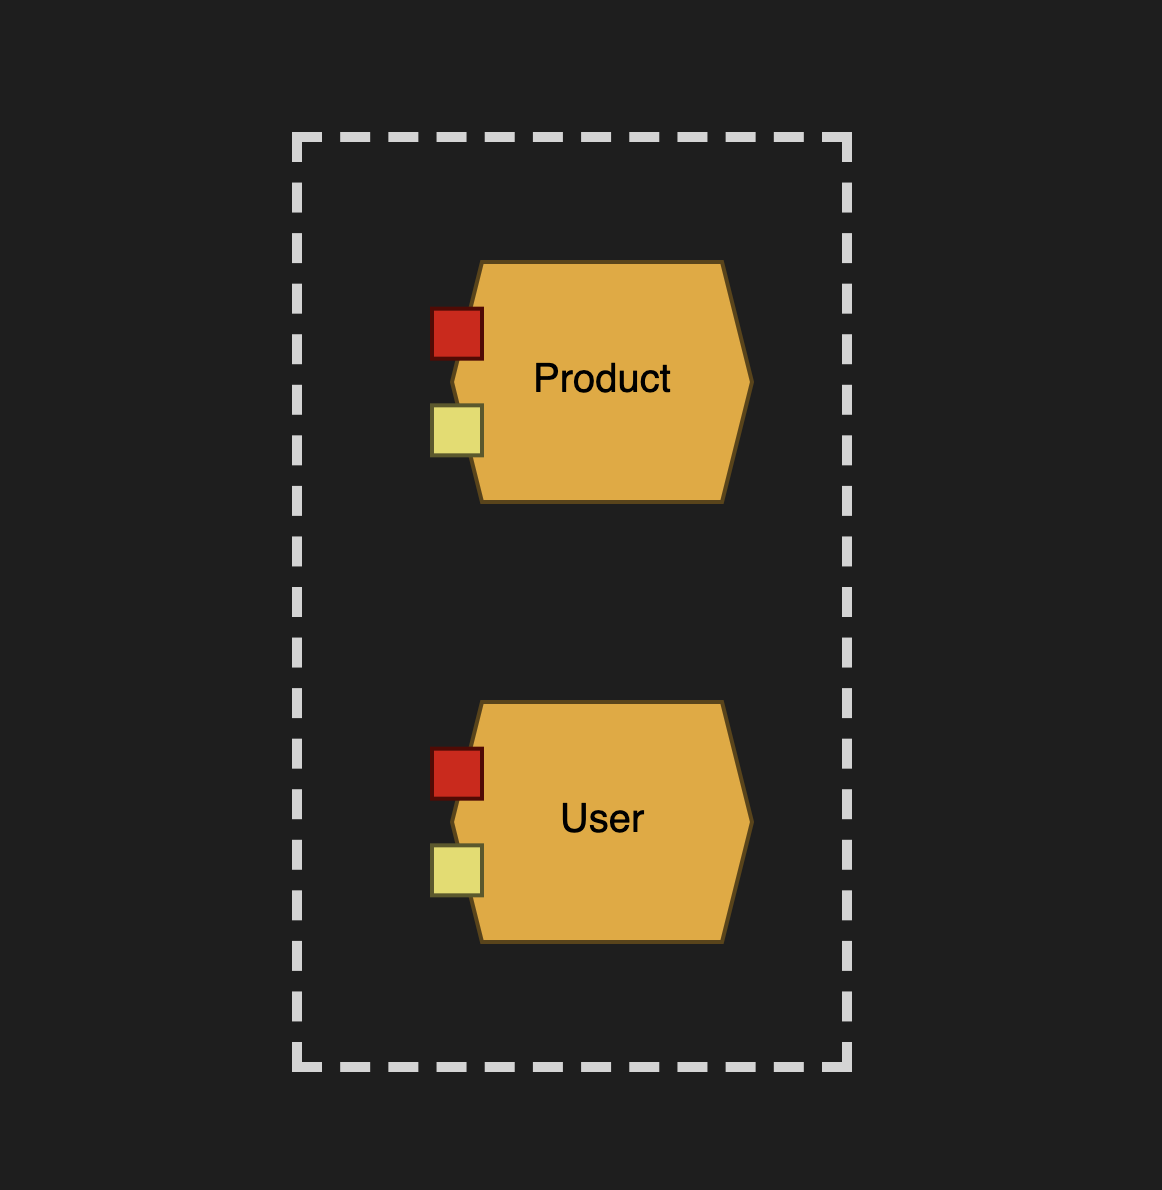
\includegraphics[width=0.5\textwidth]{figures/jv_product_and_user.png}
    \caption{The product and user services displayed in the visualization tool's UI. They have an input port (yellow) and an output port (red) each and they both are considered to be in the same network.}
    \label{figure:jv_product_and_user}
\end{figure}

The full code for the product service, types, and interface can be seen in Appendix % TODO 

\subsection{The Analytics Service}
This service supports one operation for now. This is \texttt{addToLogs(AnalyticsRequest)}, which is a one-way operation. The interface for the service is already defined, so the operation is added there with the request type being \texttt{AnalyticsRequest}. This type holds information about what content will be logged and from which service.

This service is created in the main file, and the execution is also \textit{concurrent}. The analytics service is added to the architecture file and is displayed in the visualization UI.
The input port can be created using the tool just like the last two services, and the interface for the
port is \texttt{AnalyticsIFace}.

The input port is using the TCP/IP communication medium, and the output ports in the product and user services must be connected to the input port of the analytics service.
If the ports are not connected in the visualization UI, it is possible to change the location of the ports directly in the UI.
By clicking on the ports, the sidebar will open displaying information about the ports. Double-clicking on the location field allows the user to change it.
Doing this for both output ports to make sure they have the same value in the location field will connect the output ports to the input port in the UI, as well as, change the code to match the changes made in the code.

After connecting the ports, the connections is be represented in the visualization UI. This can be seen in figure \ref*{figure:jv_analytics} where the user and product services are connected to the newly created analytics service.

\begin{figure}[h!]
    \center
    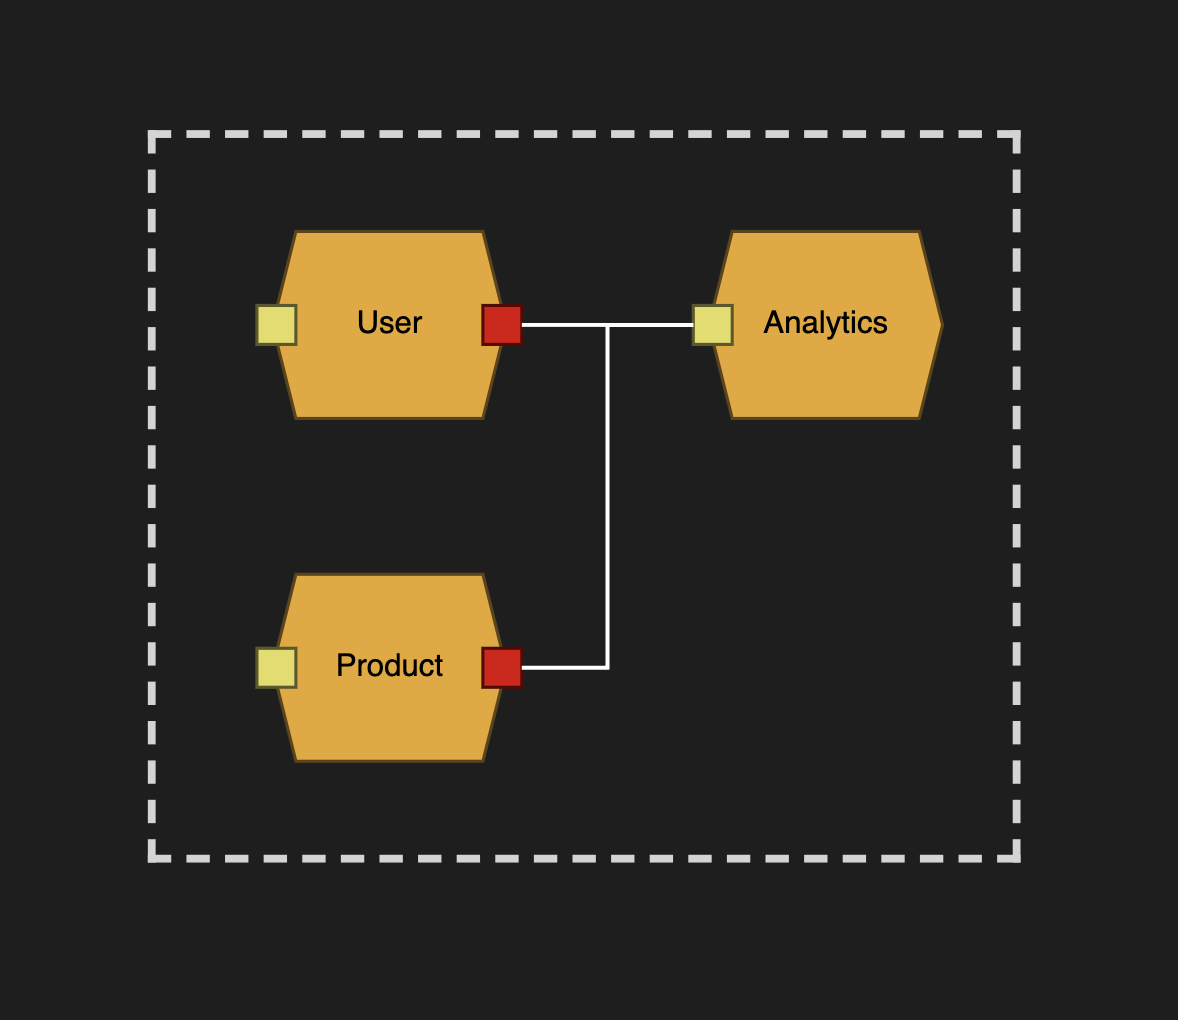
\includegraphics[width=0.5\textwidth]{figures/jv_analytics.png}
    \caption{The product, user, and analytics services displayed in the visualization tool's UI. The user and product services have an output port (red) each of which is connected to the input port (yellow) of the analytics service.}
    \label{figure:jv_analytics}
\end{figure}

\subsection{The Notification Service}
The notification service will get requests from other services and send an email to the specified user. This can be when a transaction is completed, a product is back in stock etc.
This service supports one one-way operation, \texttt{sendNotification}. The request type contains the user ID to send the notification to, and the content of the notification.
Adding the service to the architecture file will render it in the UI.

Using the UI, once again, to add an input port with the interface called \texttt{NotificationIFace}. This is the only port needed for this service.

\subsection{The Payment Service}
The payment service's only job is to process payments from orders. The interface for this service is a single request-response operation, \texttt{processPayment}.
The request type for this operation needs information about the payment method, amount to pay, user ID and credit card details. The response type has an error flag, date of purchase and optionally a receipt if the transaction was successful.

Same with all other services, this is added to the architecture file to render it in the UI. The payment service needs one input port for the interface \texttt{PaymentIFace}, an output port connected to the analytics service, and another output port connected to the notification service.
Once again, by opening the ports in the sidebar, the user can change the location of the ports to match so the correct ports are connected.

\subsection{The Order Service}
This service handles the user's orders. A user can place an order, see that order and cancel it. The interface, \texttt{OrderIFace}, has these three request-response operations: \texttt{placeOrder}, \texttt{getOrder}, and \texttt{cancelOrder}.
The request type of placing an order requires a list of products and a payment request, which could be populated by the shopping basket in the application UI.
The response type simply lets the user know if the order was placed correctly with an error flag and a status code. The "get order" operation requires an order ID of the order to return and will simply respond with an order type containing information about the order.
Cancelling an order also requires the order ID and will respond with a type with an error flag and status code.

When the order service is defined in the main file, and the service is added to the architecture file, the input port is created using the \texttt{OrderIFace} interface.
The service needs three output ports. One for the analytics service, one for the notification service and one for the payment service. The analytics that the service can log is what products get bought together and how many orders a user cancels etc.
The notification service needs to be invoked to send confirmation about cancelled orders, or if the status of the order changes.
The payment service will be invoked through the order service, so when the user places an order the payment service will get the request and send the response back to the order service which creates a response for the client.

The tool can either help in connecting the correct ports as done with the other services, but the developer can do that in the code as well, and when the developer does a change in the code manually and saves the document, the visualization UI is automatically updated to reflect the changes made in the code.

\subsection{The Recommended Service}
The last service is a standalone service, which only the client needs to invoke.
The recommended service interface consists of one request-response, \texttt{getRecommendations},
which based on the user ID given finds the most recommended products as a list of products.

A possible extension to the service can involve fetching analytics data from the analytics service and doing calculations with that information to avoid sharing databases between services. This will require the analytics service to expose an operation allowing the internal services to get the data, and an output port in the recommended service to invoke that operation.
This extension will be omitted in this example.

\subsection{The Completed Application}
With all services and ports in place, the application can be seen as one microservice architecture in the visualization UI, as seen in figure \ref*{figure:full_example_lc}.
% todo write something about inspecting the program using the sidebar
Having the whole application in the visualization tool allows the developer to inspect the application in detail to get an overview of what is happening between services and what APIs the different services expose.
Clicking on ports opens the sidebar and displays information about the ports including the interfaces. All the interfaces can be clicked on to further inspect the operations in the interface. All types used for the operations are also clickable and will display information about the type,
including the subtypes, cardinality and root type.

From here the developer can start using architectural patterns in Jolie as discussed in the previous chapter. Some refinements of the current services can also be made, for example, the payment service should probably have underlying services to take care of different payment methods.

\begin{figure}[h!]
    \center
    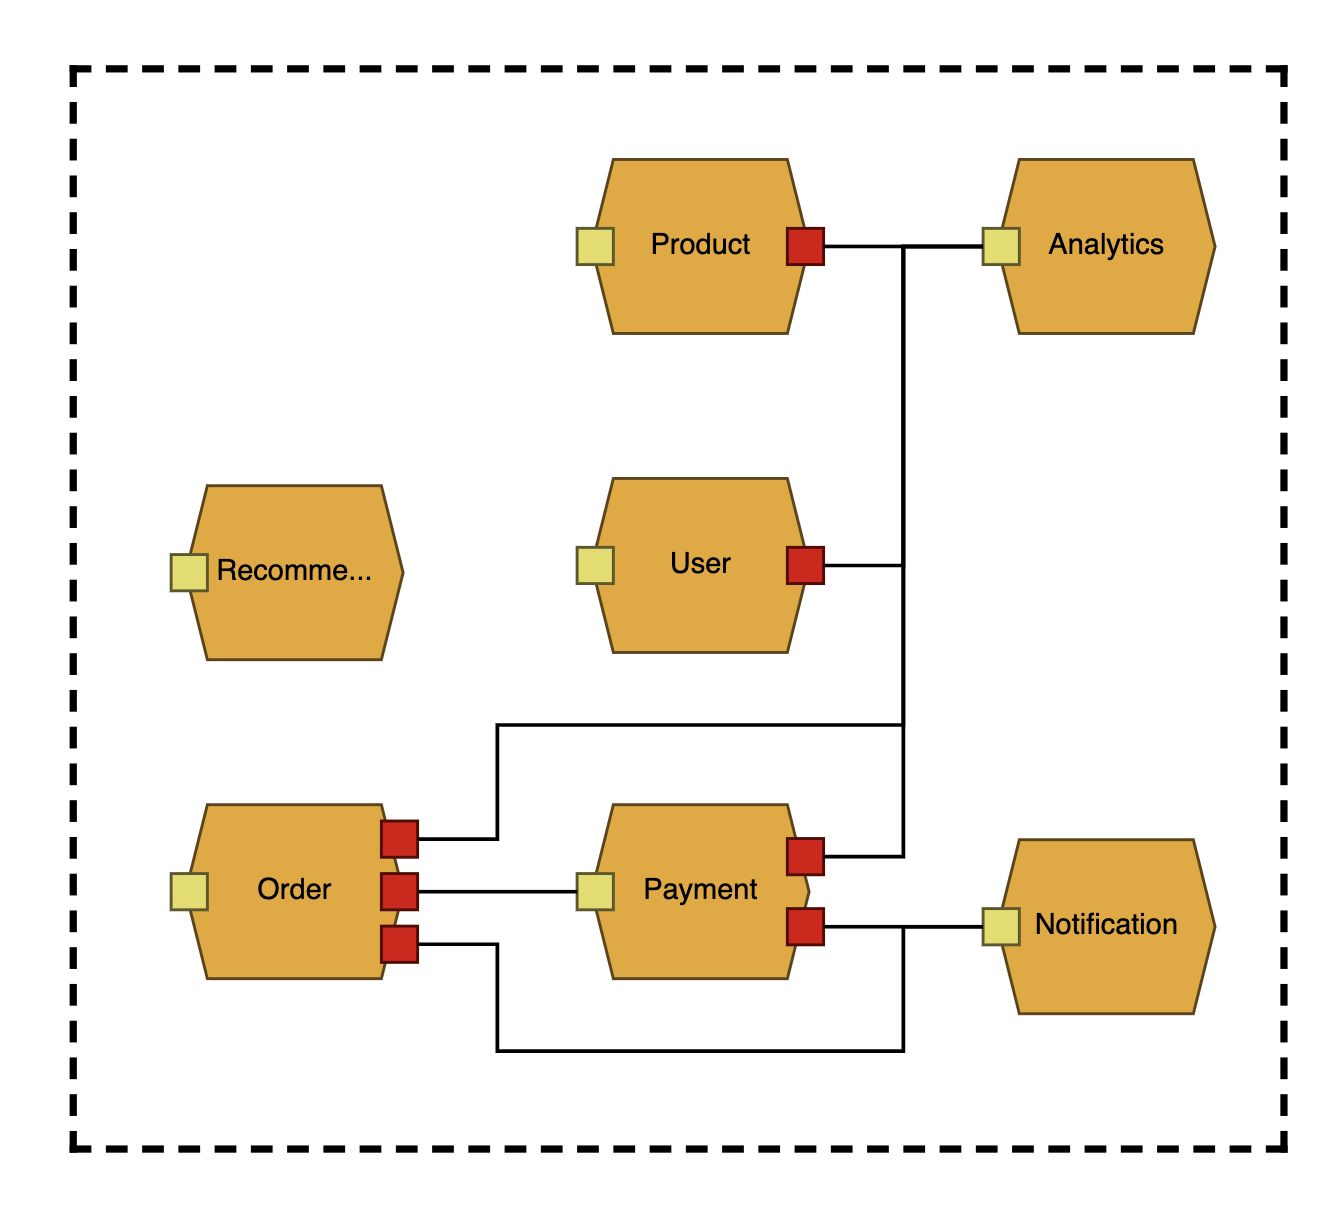
\includegraphics[width=0.8\textwidth]{figures/jv_completed.png}
    \caption{The entire e-commerce application is displayed in the visualization tool's UI. All services exist in the same network and all are top-level.}
    \label{figure:jv_completed}
\end{figure}

\section{Improvements}
Now that the application has all seven services implemented, the developer can apply some of the architectural features allowed in Jolie to improve the application and implement some of the microservices (API) patterns discussed in the last chapter.

\subsection{Embedding}
It is not necessarily the best idea to have all seven services as top-level services. The services not accessed by the client directly should be embedded in the services which need them.
The analytics service is used by four services: Order, Payment, User, and Product. To embed the analytics service in these four services the input port's location can be changed to \texttt{local}. This is just one way of embedding using local in-memory communication and is not the only way of embedding services. Another method of embedding will be used for another service later.
Changing the port location to \texttt{local} can be done in the sidebar.
The output ports in the mentioned services using the analytics interface must also be deleted which, at the moment only can be done in the code, but instead of looking for the main files which contain the ports,
opening the port in the sidebar and clicking \texttt{\{\}} at the top of the sidebar opens the correct file in the editor.

Now in the architecture file, for the analytics service, the field \texttt{instances:4} can be added to the JSON object representing the analytics service. This will add 4 instances of the analytics service, and by using the mouse and dragging the services, the developer can 
drag the services onto the four services and embed them one after one. This will add the code in the correct files to specify that the analytics service instances are embedded.

The notification service is also used by other services, and should not be accessed by a client directly. For this service, the ports will not use local in-memory communication as the analytics service did.
In the architecture file the notification service will need to have two instances, so the field for instances is added to the service JSON. Now two instances of the notification service exist as top-level services. Each instance can be dragged into its respective
parent service, namely, the order and payment services and the embedding code will be added to both services. The embedding will use the already existing ports to connect so no local ports will be created.

The last service to embed is the payment service in the order service. This can be done by either changing the existing port to use local communication or just dragging the payment service
as it is now into the order service to use the existing ports as communication and the code will again be changed to reflect the embedding.

The new architecture can be seen in figure \ref*{figure:jv_embedded} and it shows only the services which are accessed by a client. The services which now have embeddings can be seen with a little "plus" sign, which can be clicked on to expand the visualization of the service revealing local ports and embedded services.
The embedded services can be removed by dragging them out of their embedder. Doing this with local communication will cause the local ports to be removed from the code.

\begin{figure}[h!]
    \center
    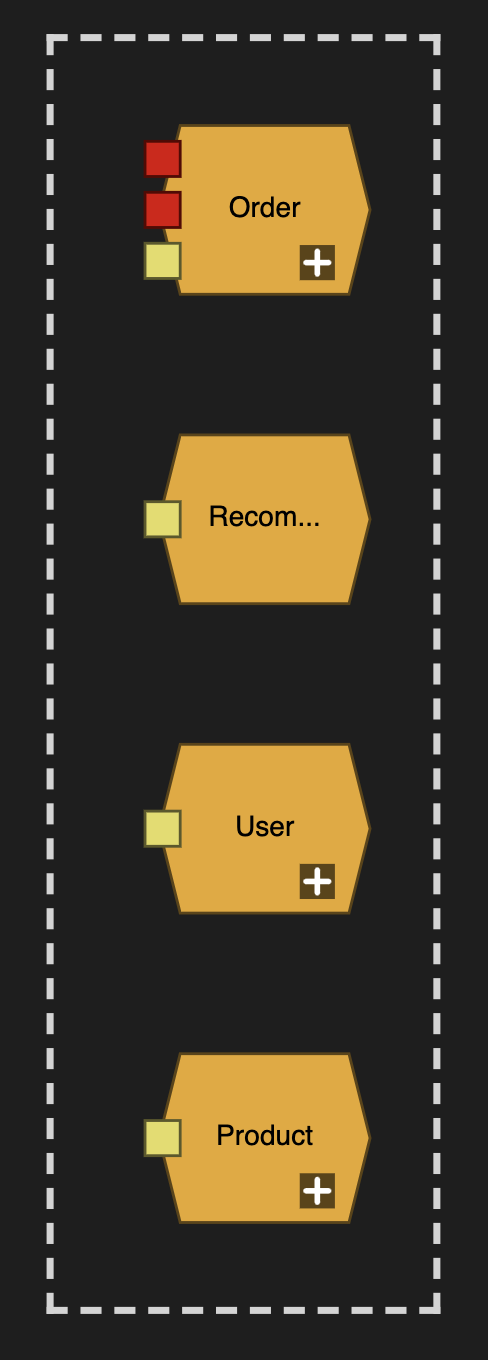
\includegraphics[width=0.2\textwidth]{figures/jv_embedded.png}
    \caption{The e-commerce application after the payment, notification, and analytics services have been embedded.}
    \label{figure:jv_embedded}
\end{figure}

\subsection{Aggregation}
Now all the top-level services are services which a client is directly requesting. It is now possible to add some of the architectural patterns to the system in order to implement some of the ideas mentioned in the previous chapter.
The tool facilitates the possibility to select services by holding the shift key and clicking the service shapes. The sidebar will show which services are selected and a list of patterns which can be applied based on some
criteria. Selecting the four top-level services of the example application shows that the aggregator pattern is applicable.

Clicking on the "aggregator" button will open a pop-up allowing the developer to enter all necessary information for creating an aggregator service, and choosing if the aggregator should connect to existing ports or create new input ports for the aggregated services, or if the aggregated services should be embedded in the aggregator service.
For this example, the aggregator will just connect using the existing ports requiring that the developer types in the locations of the input port for each service correctly.
After clicking "confirm", the aggregator service will be created in the file of the first service selected. The new architecture can be seen in figure \ref*{figure:full_example_lc} and shows that the aggregator service called \texttt{Aggregator} is connected to the services and is displayed in a slightly redder colour 
to illustrate that the aggregator is a generated service and is only a scaffolding service which the developer needs to implement the functionality for.

\begin{figure}[h!]
    \center
    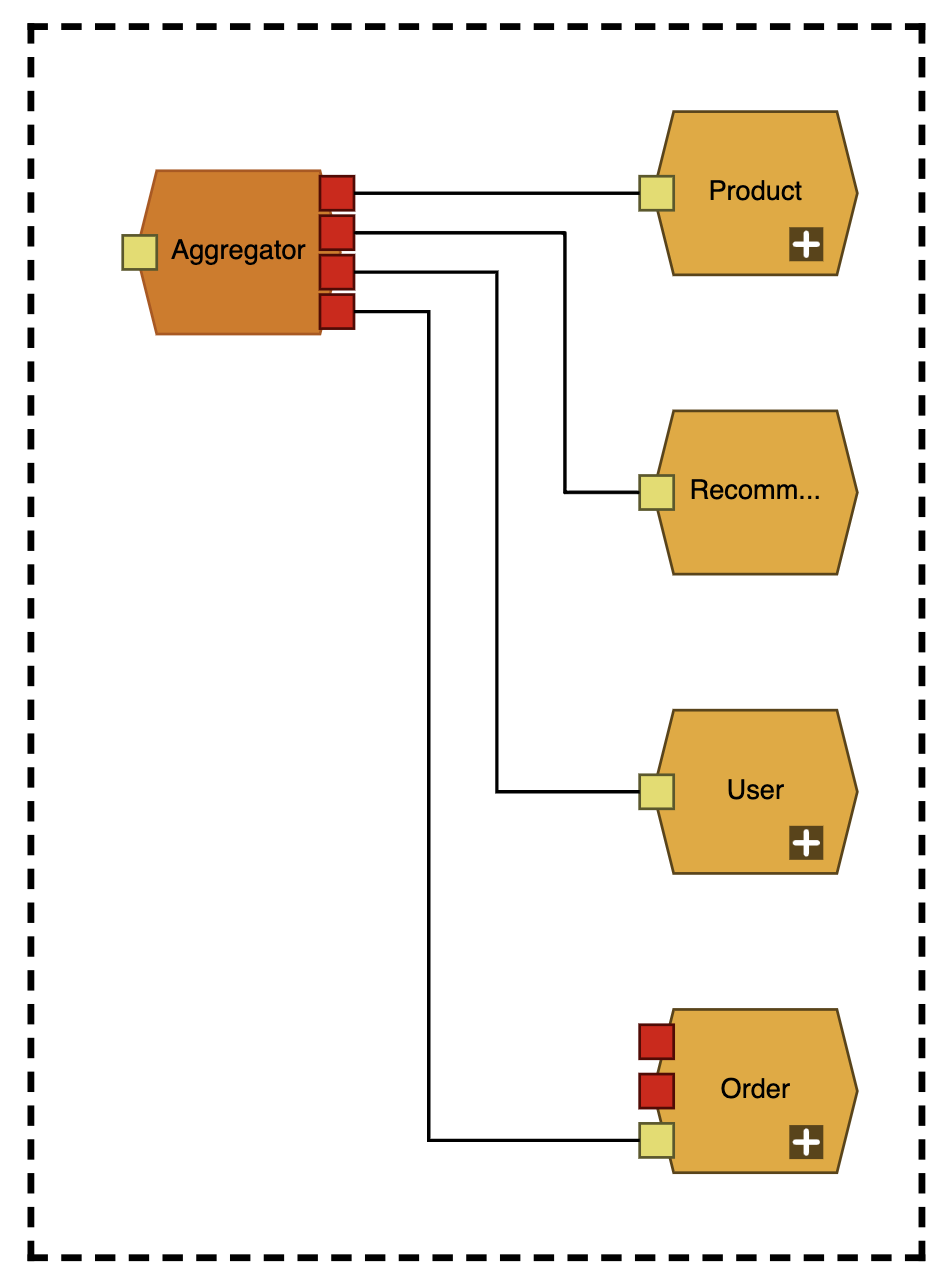
\includegraphics[width=0.41\textwidth]{figures/jv_aggregator.png}
    \caption{The e-commerce application with an aggregator service that serves as a reverse proxy for the services that are invoked by clients.}
    \label{figure:jv_aggregate}
\end{figure}

\subsection{Networks}
The final part of the application is determining which networks each top-level service belongs to. This is relevant when the application is deployed.
\section{Local Deployment}